\chapter{Selección de Objeto}

Este trabajo tiene como objetivo realizar una campaña de observación para un
sistema cuyos parámetros físicos no han sido determinados, con el propósito de
confirmar su estatus como variable cataclísmica o como una binaria eclipsante,
dependiendo del sistema y proponer una primera solución fotométrica del sistema.
Para esto, se implementó un proceso para separar e identificar objetos de
interés para observar desde el Observatorio Astronómico Universitario en
Iturbide. A continuación se describe los aspectos técnicos importantes de la
búsqueda. El código completo se encuentra en la carpeta
\href{https://github.com/KnightIV/UANL_MAPTA_Observaciones/tree/main/obsrv_plan}{\code{obsrv\_plan}},
cuyo punto de entrada se ubica en el script
\href{URLhttps://github.com/KnightIV/UANL_MAPTA_Observaciones/blob/main/obsrv_plan/main.py}{\code{main.py}}.

\section{Szkody et al. (2002): Cataclysmic Variables from the Sloan Digital Sky Survey} \label{muestra:szkody2002}

Con el lanzamiento del SDSS, Szkody y su equipo reconocieron una nueva área de
oportunidad para expandir la población de \textit{variables cataclísmicas} (VCs)
conocidas en la Galaxia. De interés particular son aquellos sistemas que más se
aproximan al periodo mínimo según los modelos evolutivos de las VCs; estos
objetos llegan a magnitudes fuera del alcance de la mayoría de los telescopios
usados hasta este entonces, por lo cual no han sido el objetivo de estudio en la
literatura. Partiendo de SDSS Szkody y colaboradores iniciaron una búsqueda de
VCs, con la expectativa de capturar una muestra representativa de
variables cataclísmicas en nuestra galaxia, en particular obteniendo muestras de
poblaciones históricamente imperceptibles a nuestros instrumentos.

Para restringir los sistemas que buscar, \citeyearparen{szkody2002CvSearchSdss}
aplicaron un criterio de color basado en el trabajo de
\citeyearparen{krisciunas1998SdssCriteria}, en el cual lograron determinar
concentraciones de diferentes tipos de objetos utilizando diagramas de
color-color. A pesar de haber hecho estas observaciones antes del año de
lanzamiento de SDSS, Krisciunas y colaboradores lograron obtener observaciones
utilizando equipo cuyas características se asemejan a las de los instrumentos
utilizados para SDSS. Partiendo de estos resultados, Szkody y colaboradores
determinaron los siguientes criterios en las regiones azules y rojas del
espectro:

\begin{equation}
	\begin{split}
		& u^* - g^* < 0.45 \\
		& g^* - r^* < 0.7 \\
		& r^* - i^* > 0.30 \\
		& i^* - z^* > 0.4
	\end{split}
	\label{muestra:szkody2002:criterioeqs}
\end{equation}

Una vez recabada la muestra de candidatas a observar, Szkody y colaboradores
confirmaron su estatus como variables cataclísmicas basado en los espectros
obtenidos del SDSS desde el \textit{Apache Point Observatory}. Estos datos los
complementaron con observaciones de espectroscopía con el telescopio de 3.5m en
el \textit{Apache Point Observatory} así como observaciones fotométricas utilizando el
telescopio de 0.76m en el \textit{Manastash Ridge Observatory} de la Universidad
de Washington. En total identificaron 22 sistemas como variables cataclísmicas,
incluyendo 3 objetos previamente estudiados e identificados como tal. Presentan
la concentración de los objetos en el diagrama color-color, vistos en la
\reffigure{szkody2002ColorColorVCs}. 

\begin{figure}[!ht]
	\centering
	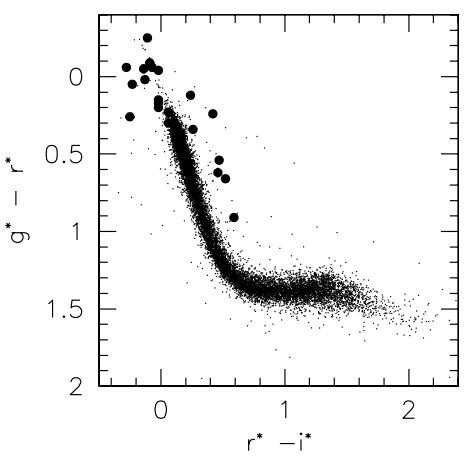
\includegraphics[scale=0.4]{Muestra/Secciones/Figures/gr-ri_Szkody2002.png}
	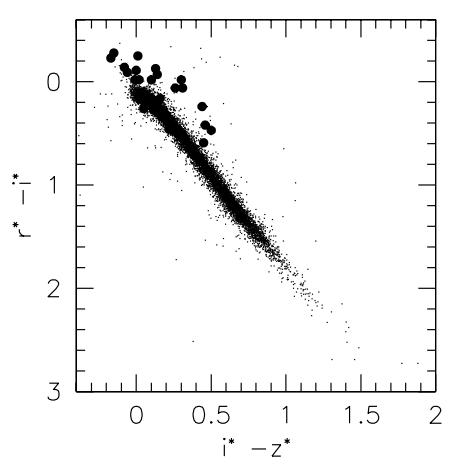
\includegraphics[scale=0.4]{Muestra/Secciones/Figures/ri-iz_Szkody2002.png}
	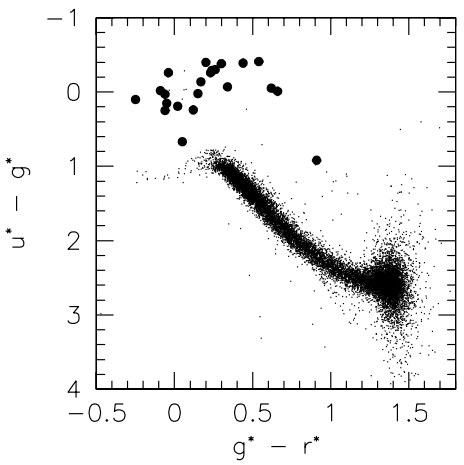
\includegraphics[scale=0.4]{Muestra/Secciones/Figures/ug-gr_Szkody2002.png}

	\caption{Variables cataclísmicas identificadas y observadas por Szkody y
		colaboradores (círculos negros fuertes). Se puede apreciar la separación
		de las variables cataclísmicas del locus estelar, vista en los puntos
		negros. \citeyearparen{szkody2002CvSearchSdss}}
	\label{szkody2002ColorColorVCs}
\end{figure}

\section{Búsqueda en Gaia}

Para obtener la muestra inicial de objetos de interés recurrimos a la base de
datos de Gaia. La selección de objetos fue llevada a cabo dentro del
\textit{Gaia Archive} utilizando su interfaz de ADQL. Los criterios
definidos por Szkody y colaboradores solo fueron definidos para el sistema
fotométrico de SDSS; para poder utilizar estos primero se llevó a cabo una
conversión de las magnitudes reportadas en el catálogo de Gaia a magnitudes en
los pasa bandas de SDSS. Esta conversión se llevó a cabo utilizando las
transformaciones definidas en la documentación de Gaia DR3
\citeyearparen{gdr3ReleaseDocumentation}, como se puede ver en la
\reffigure{gdr3SdssConversionGraphs}. Partiendo de estas magnitudes
transformadas se aplicó los criterios definidos en
\citeyearparen{szkody2002CvSearchSdss}. Sin embargo, solo dos de los 4 indices
de color se pudieron aplicar a la muestra de Gaia; no están definidas
transformaciones para las bandas $u$ ni $z$ de SDSS, ya que estas abarcan
longitudes de onda más extremas que las observadas por Gaia. El query de ADQL
ejecutada se puede encontrar en el apéndice \ref{apendice:gaiaAdql}. Se
obtuvieron en total más de \num{3630000} fuentes, el cual representa un 0.2\% de
los \num{1811709771} objetos reportados en el DR3 de Gaia. 

\begin{figure}[!ht]
	\centering
	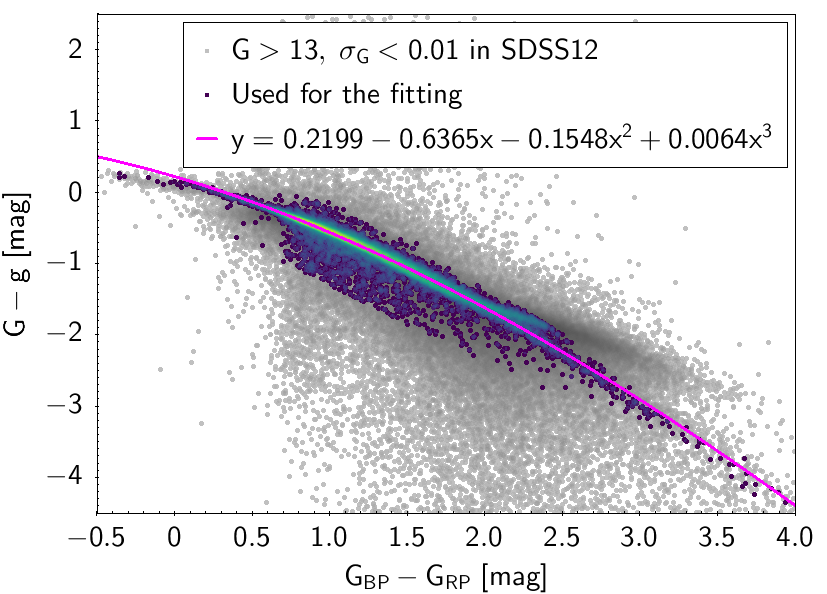
\includegraphics[scale=0.23]{Muestra/Secciones/Figures/Gaia-SDSS-Transform-g.png}
	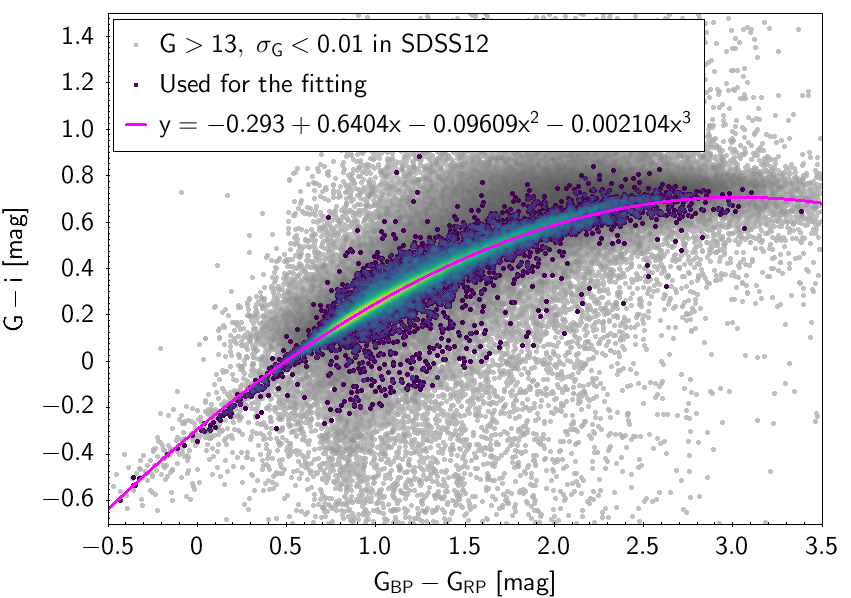
\includegraphics[scale=0.23]{Muestra/Secciones/Figures/Gaia-SDSS-Transform-i.png}
	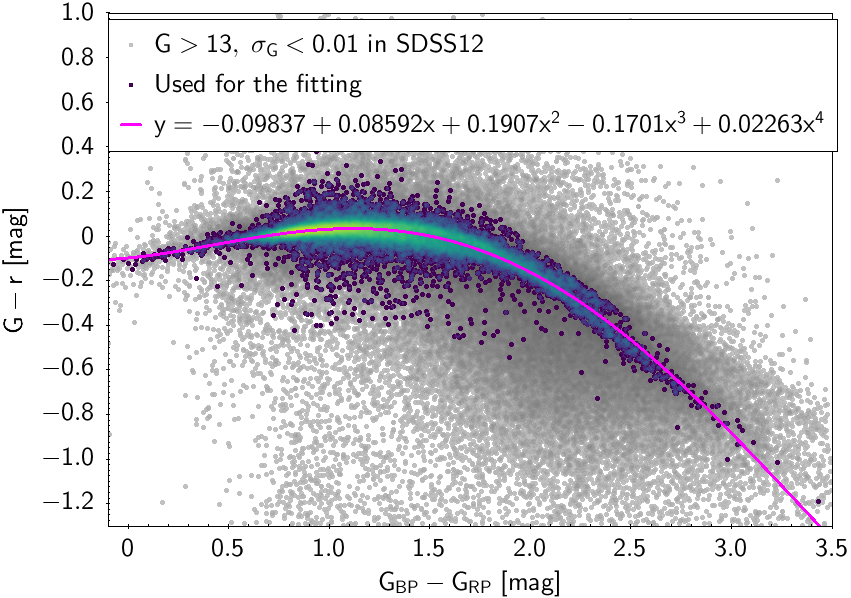
\includegraphics[scale=0.23]{Muestra/Secciones/Figures/Gaia-SDSS-Transform-r.png}

	\caption{Relación empírica entre las magnitudes reportadas en GDR3 y SDSS12.
	Las relaciones están dadas para 3 de las 5 bandas de SDSS12, debido a las
	diferencias entre las pasa bandas de Gaia y SDSS.
	\citeyearparen{gdr3ReleaseDocumentation}}
	\label{gdr3SdssConversionGraphs}
\end{figure}

\section{Selección de Objetos Observables}

La ubicación en la bóveda celeste de un sistema candidata juega un papel
importante en la viabilidad de una campaña de observación desde el OAU. Esto
determina si un objeto es visible desde la locación geográfica del observatorio
durante las fechas de observación; de otra manera sería imposible apuntar un
telescopio al sistema. Para realizar esta tarea se utilizaron los módulos de
\code{astroplan} \citeyearparen{astroplan} y \code{astropy} \citeyearparen{astropy}, aplicando
el algoritmo a los objetos resultados de la búsqueda en la base de datos de
Gaia. El código responsable se encuentra en el archivo
\href{https://github.com/KnightIV/UANL_MAPTA_Observaciones/blob/main/obsrv_plan/gaia/observable_targets.py}{\code{observable\_targets.py}}.

\section{Búsqueda en SIMBAD}

Una vez obtenidos los objetos de interés de la selección de objetos visibles se
utilizó la base de datos de
SIMBAD\footnote{\url{http://simbad.cds.unistra.fr/simbad/}}
\citeyearparen{simbadDatabase} para restringir los objetos de interés a un
tamaño manejable, con el objetivo de obtener un sistema clasificado como
variable cataclísmica, binaria eclipsante, o candidata a alguna de estas
clasificaciones. Uno de los objetivos de este trabajo de tesis fue realizar una
campaña de observación al sistema elegido, con finalidad de obtener una curva de
luz fotométrica; por lo tanto, un requisito para este trabajo de maestría es que
este sistema sea uno con una cantidad minima de estudios antecedentes; el
estudio del sistema dependerá en gran parte de la curva de luz obtenida de las
observaciones. El código que llevó a cabo esta búsqueda se encuentra en
\href{https://github.com/KnightIV/UANL_MAPTA_Observaciones/blob/main/obsrv_plan/simbad/categorize_all_targets.ipynb}{\code{categorize\_all\_targets.ipynb}},
cuyos resultados se pueden ver en la \reffigure{figuraBusquedaSimbadHistograma}.
Las estrellas variables de largo periodo (\code{LongPeriodV*} y las candidatas
\code{LongPeriodV*\_Candidate}) que consisten predominantemente de estrellas
pulsantes son las que representan la mayoría de objetos obtenidos de la búsqueda
en Gaia. Varios de las fuentes de GDR3 no tienen algún estudio antecedente que
SIMBAD tenga registrado en su base de datos; de los \num{3630000} resultados,
solo fue posible conseguir la clasificación de \num{997199} objetos
individuales. De aquellos resultados clasificados como candidatos a binarias
eclipsantes se escogió un objeto visible desde el \textbf{Observatorio
Astronómico Universitario} en Iturbide, N.L., descrito en la
\refthesissection{muestra:observaciones:oau}.

\begin{figure}[!ht]
	\centering
	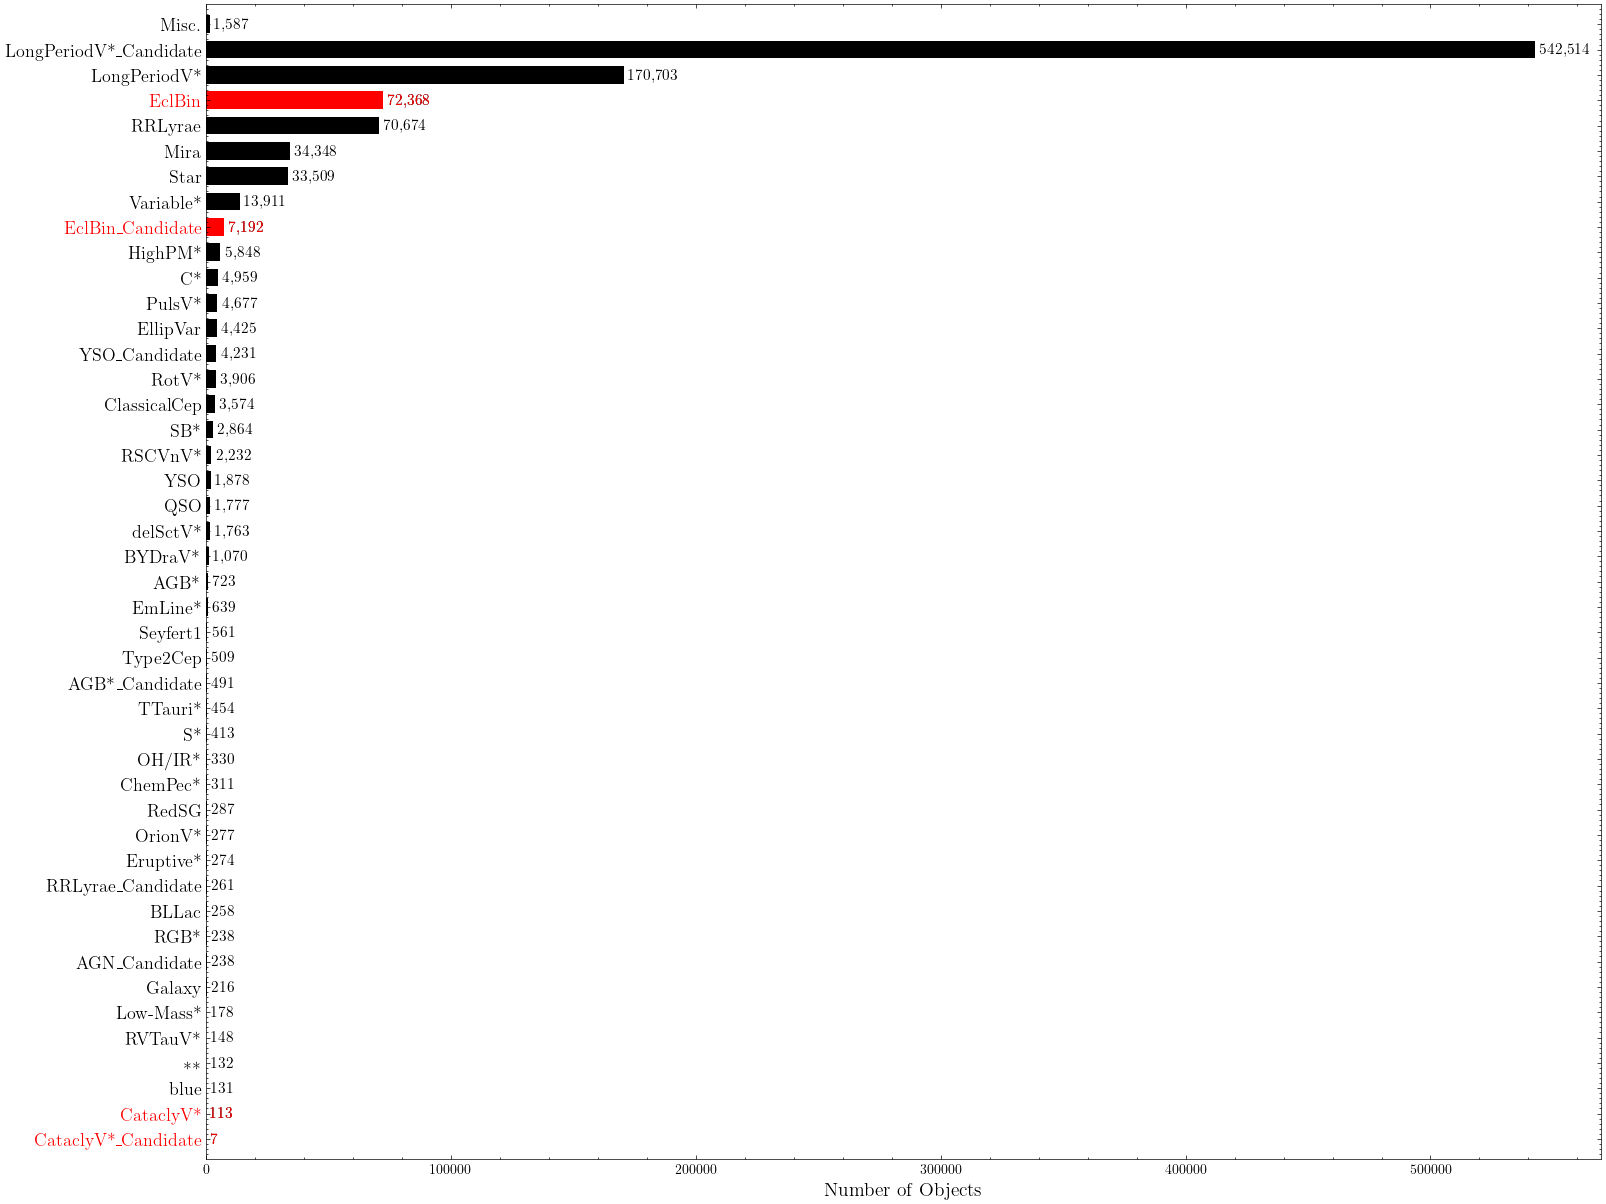
\includegraphics[scale=0.4]{Muestra/Secciones/Figures/Figura Gaia SIMBAD Busqueda Resultados.png}
	\caption{Histograma de las clasificaciones de los objetos capturados en la
	búsqueda dentro del catálogo GDR3, haciendo un análisis cruzado con la base
	de datos de SIMBAD. En rojo se resaltan las categorías de principal interés:
	los sistemas \textit{binarias eclipsantes} (\code{EclBin}) junto a las
	\textit{candidatas a binarias eclipsantes} (\code{EclBin\_Candidate}), e
	incluyendo sistemas de tipo \textit{variable cataclísmica} (\code{CataclyV*}
	y las candidatas \code{CataclyV*\_Candidate}), un tipo en particular de
	sistemas binarios en semi contacto
	\citeyearparen{smith_cataclysmic_variables_review_2007}. Varias
	clasificaciones de baja importancia quedan agrupadas en la categoría
	\code{Misc.} por brevedad.}
	\label{figuraBusquedaSimbadHistograma}
\end{figure}

\section{ATO J339.9469+45.1464 - EclBin}

\citeyearparen{atlasATOObjectDiscovery} realizaron una búsqueda de estrellas
variables dentro de la primera publicación de datos del catálogo
\textbf{Asteroid Terrestrial-impact Last Alert System} (\textbf{ATLAS}), el cual
contiene las observaciones realizadas por el telescopio Haleakalā durante los
primeros 2 años de operación hasta finales de Junio del 2017, aprovechando su
cobertura de aproximadamente \num{13000} $\mathrm{deg}^2$ al menos 4 veces por
noche. Esta cadencia de observación es ideal para observar estrellas variables;
el tiempo de observación es suficientemente corto para obtener una curva de luz
adecuada para estudiar estos sistemas. Lograron clasificar las estrellas
variable del catálogo en 15 distintas categorías dependiendo de la morfología de
sus curvas de luz; de estas reportan que \num{74700} fuentes son binarias
eclipsantes. A pesar de haber confirmado la clasificación de estas fuentes, aún
quedan varios sistemas cuya naturaleza es desconocida.

\textbf{\atoObjId} está clasificado como una de estas candidatas a binaria
eclipsante. Como este sistema carece una clasificación concreta, no existe mucha
información acerca de ella. Tiene una magnitud promedio de aproximadamente
\num{16.91}, lo cual lo hace un sistema tenue. Con una ascensión recta de
\code{22 39 47.2569} y declinación de \code{+45 08 47.0311}, \atoObjId
es un sistema ideal para observar desde el OAU en Iturbide.

Antes de terminar este trabajo de maestría pero después de haber seleccionado al
objeto \atoObjId para estudiar, su clasificación en SIMBAD cambió a ser una
binaria eclipsante confirmada.
\citeyearparen{chen_ztf_catalog_periodic_variable_stars_2020} utilizaron los
datos dentro del Data Release 2 del catálogo de ZTF para clasificar varios tipos
de estrellas variables utilizando una metodología para identificar y clasificar
objetos hasta una magnitud de 20.6. Sin embargo, este estudio solo llegó a
clasificar el sistema; este trabajo de tesis profundiza el estudio para este
sistema, llegando a una solución fotométrica para determinar los parámetros
físicos del sistema.

\subsection{Datos de Gaia}

Como parte de sus observaciones regulares, Gaia ha observado \atoObjId durante 3
años de operación, obteniendo magnitudes del sistema en varias etapas en su fase
empezando desde agosto del 2014 hasta mayo del 2017. En la
\reffigure{gdr3AtoObjLightCurves} se pueden ver las 3 curvas de luz de Gaia en
cada pasabanda, $G_{\mathrm{BP}}$, $G_{\mathrm{RP}}$ y $G$. Estas mediciones en distintos filtros
permite el análisis del color del sistema, el cual permite ajustar la
temperatura efectiva de una solución fotométrica a los datos observados. Este
método de determinar las temperaturas efectivas del sistema no solo nos libra de
tener que utilizar una relación empírica para darle como dato de entrada al
modelo\textemdash un ajuste de mínimos cuadrados tendrá que tomar en cuenta la
física de radiación de ambas componentes durante cualquier proceso de
optimización de parámetros\textemdash pero también permite determinar la
incertidumbre de este parámetro por medio del muestreo del espacio de parámetros
libres.

% TODO: maybe move to appendix?
\begin{figure}[!ht]
	\centering
	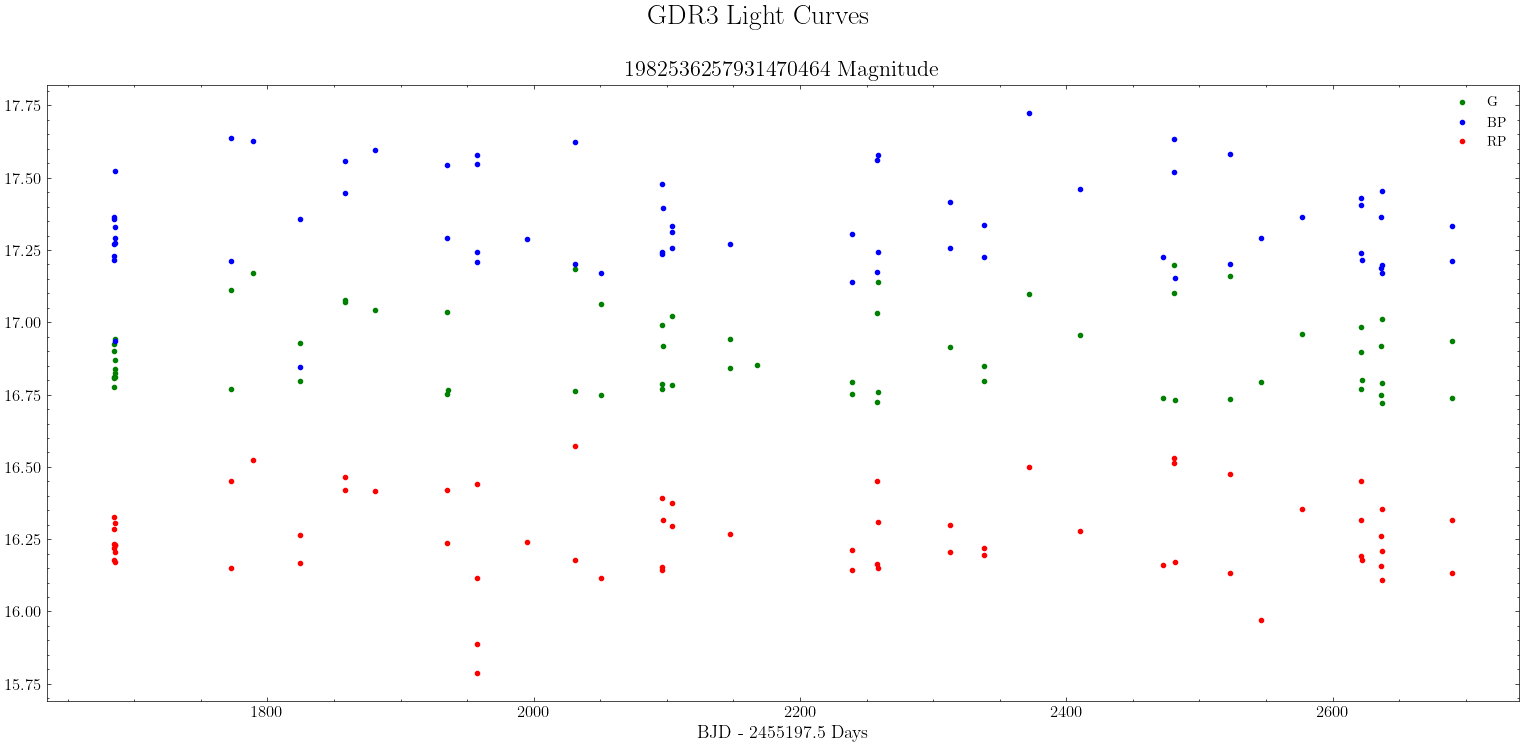
\includegraphics[scale=0.42]{Muestra/Secciones/Figures/GDR3-Light-Curves.png}
	\caption{Magnitud de \atoObjId registrada en la base de datos de Gaia DR3
	bajo su número identificador en el catálogo. Se puede apreciar la
	variabilidad de aproximadamente 0.5 mag en el brillo del sistema, la cual la
	atribuimos a la presencia de eclipses en el sistema binario. Las tres curvas
	de luz corresponden a cada pasabanda de la misión de Gaia: verde es la banda
	$G$, en azul la banda $G_{BP}$, y en rojo la banda $G_{RP}$.
	[\citeyearparen{gdr3ReleaseDocumentation}]}
	\label{gdr3AtoObjLightCurves}
\end{figure}

\subsection{Datos de ZTF}

Las curvas de luz de Gaia DR3 ofrecen mediciones con una precisión nunca antes
vistas. Sin embargo, el enfoque de la misión es en el cálculo de las propiedades
astrométricas de los objetos observados (incluyendo posiciones angulares,
velocidades propias, etc.); el producto principal de la misión no son las curvas
de luz fotométricas. La cadencia de observación resulta en una resolución
temporal pobre del sistema. Una dificultad adicional en el análisis de PHOEBE es
el trato de la extinción interestelar, ya que por cuestiones técnicas PHOEBE no
puede generar un modelo sintético para ciertas pasabandas cuando se aplica el
efecto de extinción interestelar; por ejemplo, PHOEBE puede calcular un
modelo que cuenta con curvas de luz en los 3 pasabandas de Gaia, pero no puede
generar una curva sintética para un modelo en las pasabandas de ZTF. Las tablas
de atmósferas estelares que PHOEBE utiliza no tienen la información necesaria
para extinguir de manera adecuada la radiación emergente para cada pasabanda.
En el caso de las curvas de luz de GDR3 esto llega a ser un problema
significativo cuando se tiene un coeficiente de extinción $E(B - V)$ apreciable,
debido a que afecta principalmente a cortas longitudes de onda.

Para complementar la información de color obtenida de Gaia y obtener una curva
de luz con alta resolución temporal\textemdash y una alta cobertura de la curva
de luz en fase\textemdash se realizó una búsqueda de datos en el catálogo de
ZTF, en particular el \textit{Data Release 20} la última versión de los datos
publicados durante la fase de recolección de datos del proyecto. Para \atoObjId
se obtuvieron 2 curvas de luz en las bandas ZTF:g y ZTF:r, las cuales no han
sido corregidas para tomar en cuenta el color del sistema en el procesamiento
hecho por IRSA. Las observaciones de ZTF se registraron desde el 20 de abril del
2018 hasta el 2 de julio del 2023 para el filtro ZTF:g, y desde el 17 de mayo
del 2018 hasta el 2 de julio del 2023 para el filtro ZTF:r. Las curvas de luz
completas se pueden ver en la \reffigure{figuraZtfCurvasLuz}.

% TODO: maybe move to appendix?
\begin{figure}[!ht]
	\centering
	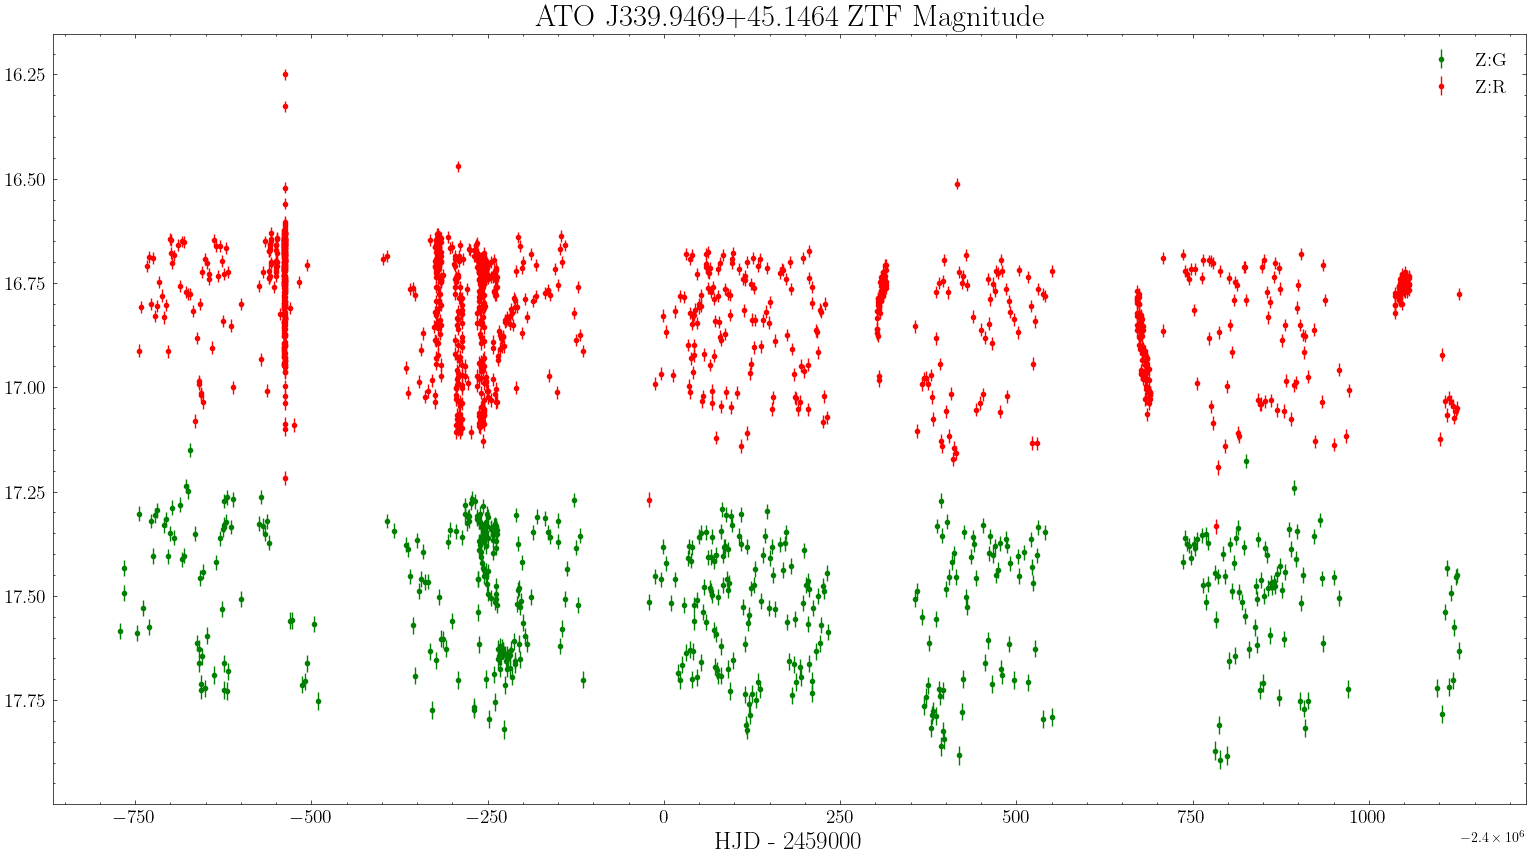
\includegraphics[scale=0.42]{Muestra/Secciones/Figures/Figura ZTF Light Curves.png}
	\caption{Curvas de luz en las pasabandas ZTF:g (verde) y ZTF:r (rojo) para \atoObjId, 
	obtenido del catálogo de ZTF por su identificador de SIMBAD.}
	\label{figuraZtfCurvasLuz}
\end{figure}